\documentclass[oldfontcommands]{MScthesisITEM}

\usepackage{amsthm}
\usepackage{float}
\usepackage{fancyvrb}
\usepackage{listings}
\usepackage{wrapfig}



\title{Exploring CryptDB:\newlinetitle A Practical HE Scheme for SQL Queries} % The title of your assignement; NB use \newlinetitle to start a newline
\author{Eirik Klevstad} % Your firstname and lastname
\professor{Colin Boyd, ITEM} % Affiliation = ITEM for instance
\supervisor{Chris Carr, ITEM}

%% Uncomment the following in case you want subfigures; note that there will be a warning for the caption package
% \let\subcaption\undefined
% \let\subfloat\undefined
% \usepackage[bf]{caption}
% \usepackage{subcaption}

\DeclareGraphicsExtensions{.pdf,.jpg}
\graphicspath{{./figs/}}

\loadglsentries{glossary}
\makeglossaries

\begin{document}
\selectlanguage{english}
\pagenumbering{roman}
\pagestyle{plain}


%% Only for the project; comment out the line below for the master's thesis; the front page will be generated automatically by DAIM
\titleITEM

%% Only for the master's thesis; for the project report the description is taken from It's Learning and added by the department
% \selectlanguage{english} % Change to 'norsk' if you are writing in Norwegian
% \begin{titlingpage}

\noindent
\begin{tabular}{@{}p{4cm}l}
\textbf{Title:} 	& \thetitle \\
\textbf{Student:}	& \theauthor \\
\end{tabular}

\vspace{4ex}
\noindent\textbf{Problem description:}
\vspace{2ex}

\noindent \Blindtext[2][1]
\vspace{6ex}

\noindent
\begin{tabular}{@{}p{4cm}l}
\textbf{Responsible professor:} 	& \theprofessor \\
\textbf{Supervisor:}			& \thesupervisor \\
\end{tabular}

\end{titlingpage}
% \cleardoublepage

%% There must be an abstract in English, even though the main text is in Norwegian
\selectlanguage{english}
\pagestyle{empty}
\begin{abstract}
\noindent This is an awesome abstract.
\end{abstract}
\cleardoublepage

%% Only for the master's thesis; if the main text is in English and you can write Norwegian, there must be an abstract in Norwegian as well.
% \selectlanguage{norsk}
% \pagestyle{empty}
\renewcommand{\abstractname}{Sammendrag}
\begin{abstract}
\noindent Sikkerheten til nesten all offentlig nøkkel-kryptografi er basert på et vanskelig beregnbarhetsproblem. Mest velkjent er problemene med å faktorisere heltall i sine primtallsfaktorer, og å beregne diskrete logaritmer i endelige sykliske grupper. I de to siste tiårene, har det imidlertid dukket opp en rekke andre offentlig nøkkel-systemer, som baserer sin sikkerhet på helt andre type problemer. Et lovende forslag, er å basere sikkerheten på vanskeligheten av å løse store likningsett av flervariable polynomlikninger. En stor utfordring ved å designe slike offentlig nøkkel-systemer, er å integrere en effektiv ``falluke'' (trapdoor) inn i likningssettet. En ny tilnærming til dette problemet ble nylig foreslått av Gligoroski m.f., hvor de benytter konseptet om kvasigruppe-strengtransformasjoner (quasigroup string transformations). I denne masteroppgaven beskriver vi en metodikk for å identifisere sterke og svake nøkler i det nylig foreslåtte multivariable offentlig nøkkel-signatursystemet MQQ-SIG, som er basert på denne idéen.

Vi har gjennomført et stort antall eksperimenter, basert på Gröbner basis angrep, for å klassifisere de ulike parametrene som bestemmer nøklene i MQQ-SIG. Våre funn viser at det er store forskjeller i viktigheten av disse parametrene. Metodikken består i en klassifisering av de forskjellige parametrene i systemet, i tillegg til en innføring av konkrete kriterier for hvilke nøkler som bør velges. Videre, har vi identifisert et unødvendig krav i den originale spesifikasjonen, som krevde at kvasigruppene måtte oppfylle et bestemt kriterie. Ved å fjerne denne betingelsen, kan nøkkel-genererings-algoritmen potensielt øke ytelsen med en stor faktor. Basert på alt dette, foreslår vi en ny og forbedret nøkkel-genereringsalgoritme for MQQ-SIG, som vil generere sterkere nøkler og være mer effektiv enn den originale nøkkel-genereringsalgoritmen.  
\end{abstract}
% \cleardoublepage

\selectlanguage{english}% Change to 'norsk' if you are writing in Norwegian

\renewcommand{\abstractname}{Preface}
\begin{abstract}
\noindent \blindtext 
\end{abstract}
\cleardoublepage

% similarly you may add a separate acknowledgments page

\tableofcontents*
\cleardoublepage

%% include if relevant
\listoffigures
\cleardoublepage

%% include if relevant
\listoftables
\cleardoublepage

%% include if relevant
%\listofalgorithms
%\addcontentsline{toc}{chapter}{List of Algorithms}
%\cleardoublepage

%% include if relevant
%\printglossary[title=List of Symbols, style=long]
%\cleardoublepage
%\glsaddall[]

%% include if relevant
\printglossary[title=List of Acronyms,type=\acronymtype] % prints just the list of acronyms
\cleardoublepage

\pagenumbering{arabic}
\pagestyle{ruled}

\chapter{Introduction}
\label{chp:introduction}

\section{Motivation}

Cloud services are becoming larger and more complex. Users want their content available wherever they are, forcing applications to store content in the cloud. Companies such as Apple \cite{apple_health}, Microsoft \cite{microsoft_health} and other corporations are looking into health information and how your personal information can be integrated into their services. Medical research facilities stores tremendous amounts of personal data, and are currently looking into how to share their research material across facilities and borders. Along with these types of sensitive data, follows great responsibility and security measures. When developing applications and systems, data security and confidentiality are important topics.

% Bør reformulere setningen som starter med iDASH til å starte med noe annet.
% One of the iDASH \cite{iDASH} leads on into combining biomedical research and technology. 

As a developer, you are left with two choices. Option one is to build our own server farm or data center on a secure site, which is a rather expensive solution with costs related to both hardware, maintenance, electricity and rent. Option two is to out-source the storage to a cloud provider, where the developer stumbles into another problem. How can we guarantee that the data is stored securely, given that we cannot necessary trust the provider.

The first solution that comes to our mind is that the user could encrypt its data with a strong block cipher, and then decrypt the result at the client side. Sure, but this does not really solve anything. Problems arise when the application needs to perform operations that are too heavy for an ordinary client's machine. What if there existed a database system that could solve these problems for us? A system where the data is safely stored in the cloud without the possibility of having database administrators snooping around, or adversaries able to extract any information in the (un)likely case of a database breach. A system that could perform all kinds of operations on our data and send the encrypted result back, without leaking any sort of information about the query, the result, the data itself or any intermediate values. Homomorphic encryption schemes might be our rescue.

In short terms, homomorphic encryption is a cryptographic property describing the ability to perform certain operations on encrypted data (ciphertexts) without decrypting it first. Fully homomorphic encryption is the enhanced version where the encryption scheme is capable of performing all efficient functions \cite{Gentry_thesis}. While still in research mode, fully homomorphic encryption schemes' biggest challenge is efficiency. As for practicality, fully homomorphic encryption schemes still have a long way to go \cite{naehrig2011can}.

Something more specific about CryptDB and why it is interesting. Its key ideas.

Maybe we can achieve FHE in another way?

For now: What is practically possible?

\section{Problem}

Describe the problem/objective.\\
The aim of the project.
Short explanation of results

\section{Scope}

Any differences from the project description goes here. Redefine. Explain.

\section{Related Work}

To be continued. 

\chapter{Background}
\label{chp:background}

This chapter will cover the cryptographic background of the necessary components in order to understand CryptDB, along with some of the basic cryptographic principals.

...More. Symmetric/Asymmetric/ has no references. Is this trivial enough to go without?


% Generelt om databaser.

\section{Databases and Database Systems}

Databases are central building blocks in most computer systems, allowing data to be stored, shared, and read by users. When we want to save our data, we need a place to store it. Formally, databases can be described as a set of related data that us organized in such a way that data can easily be accessed, managed, and updated. As the amount of data stored does not decrease over time, database systems experience an exponential growth and are becoming more and more complex.

Databases are often constructed of one or more \emph{tables} which consists of multiple \emph{fields} or columns as seen in Figure \ref{fig:db_table}. These columns are usually defined to store values of some predetermined \emph{data type}, for example integers, dates, strings or decimals. 

\begin{figure}[h]
	\centering
	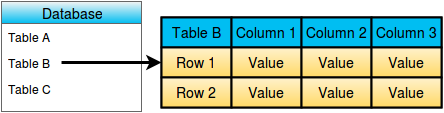
\includegraphics[scale=0.7]{db_table.png}
	\caption{A table within a database consists of multiple columns, when inserting values into a table, a new row will be created storing the data}
	\label{fig:db_table}
\end{figure}

\gls{dbms} are software used to enable clients and applications to interact with a database. These systems are often classified based on the database model they support, which is a logical structure describing the database as well as determining the permitted ways of storing information. The, possibly, most popular model is the relational database, mostly because of it being the main model for large \gls{dbms} such as MySQL, PostgreSQL, Oracle and Microsoft SQL Server.

Now we got a \gls{dbms} with a database storing some tables with our data. How do we put data in our database, and how do we extract data from it? In order for databases do anything useful other than just storing the data, they need a query language. A query language is used by \gls{dbms} to insert and extract data from databases. \gls{sql} is the standard language for performing queries on relational databases, which enables systems to insert, update and delete data, as well as performing functional operations such as summation, average, and finding maximum and minimum values.

\subsection{Database Security}
\label{chp:database_Security}

Databases are central building blocks in most computer systems, allowing data to be stored, shared, and read by users. As the amount of data stored does not decrease over time, database systems experience an exponential growth. There are companies that stores banking information, health records, and other sensitive information, which makes them a target for criminals and hackers. In order to cope with such attacks, systems that are relying on some sort of database structure, are in need of defence mechanisms. 


Most database systems are stored behind different network security measures such as firewalls and intrusion detection systems. A database firewall will, for example, monitor all traffic to and from a database system in order to detect situations that deflects from the predetermined database policy. Such measures does however only provide security for the outside of the system, but a system is in need of security on the inside as well. Most database systems provide different security measures for handling situations that can occur on the inside.

Access control is used for granting different privileges for a user or user groups to a certain object in the database, such as a table, view or procedure. Authentication is used to ensure that only trusted entities are able to reach the database, and to grant the correct privileges based on the identity of the user. For applications where certain user groups are handling sensitive information, a person in charge of the system may have the need to monitor who accessed a given table at a certain time in case of information leaks and similar circumstances. Auditing is a database security technique which does not directly prevent security protocols from being broken, but allows the system administrator to backtrack and discover breaches in the security.

Another vital part of keeping a database secure, is of course the use of database encryption. Both symmetric and asymmetric encryption is possible to perform on database systems, and there exists different ways of layering the encryption based on the application.


Hmm. Not sure about how good this section is. What to add, remove, etc?

\section{Symmetric Encryption}

Symmetric key encryption is, perhaps, the most intuitive type of encryption, where the sender encrypts the data with a secret key that the sender and receiver has agreed upon in advance. When receiving data, the receiver uses the pre-shared secret key in order to decrypt the data. In a more formal matter, symmetric key encryption is usually used either with a block cipher(which encrypts messages in chunks of data) or a stream cipher (which encrypts data bit-by-bit). The scheme usually consist of three algorithms, $KeyGen$, $Enc$ and $Dec$.

$KeyGen$ is the algorithm that generates the secret key $k_s$ used for encryption and decryption, $Enc_k$ encrypts the data with the secret key, and $Dec_k$ decrypts it using the same secret key. One of the major drawbacks with symmetric key cryptography is that the secret key $k_s$ needs to be shared between the parties that are communicating. If an adversary obtains the secret key, say that one of the parties stored it on a piece of paper that was misplaced and lost, the whole communication channel would be compromised as the adversary could easily decrypt the data.

In database systems, symmetric encryption is often used to store data by encrypting it under some secret key $k_s$ that is kept in the database. Given that the information in the database is stored using the same key, this approach provides little security against unauthorized users that gain access to the secret key. On the plus side, the process of encrypting data using a symmetric encryption scheme is usually fast compared to other approaches that uses multiple keys.


\section{Asymmetric Encryption}

In contrast to symmetric key encryption, asymmetric key encryption does not depend on a pre-shared secret key. Asymmetric key encryption, or Public-Key Encryption, is based upon the fact that some mathematical problems are considered \emph{hard}, such as the integer factorization, discrete logarithms and elliptic curves. By computing a key-pair consisting of a public key and a private key, two users are able to exchange keys over a public channel without worrying about their secret keys being compromised.

The public key is used for encrypting data sent to the user, and the private key is used to decrypt received data that is encrypted with said public key. Two of the most recognized public-key cryptosystems are \gls{rsa}, which relies of the integer factorization problem, and ElGamal, which relies on the discrete logarithms problem. In addition to secure communication between multiple parties, public key cryptography is also applied to create digital signatures, which provides authentication and data integrity.

For applications using databases that are storing information for different users, asymmetric encryption would be a natural encryption scheme. Information sent from one user to another could be encrypted under the receivers public key and vice-versa, and decrypted by applying their secret keys.

% Why are we talking about asymmetric encryption?

\section{Homomorphic Encryption}

We love to describe encryption as safes where we store our data, then secures it with one or more locks, and hide the secret key. Without the secret key, the data is securely stored inside the safe. Whenever we need our data, we take the hidden key out from its hideout and opens all the locks of the safe, where the data is as intact as we left it. The, perhaps, holiest of all the holy grails in cryptography is called \emph{homomorphic encryption}. This is a special case of encryption where operations on the encrypted data are possible without decrypting it first, or in the perspective of our locked safe: Modify the data on the inside of the safe without ever unlocking it. Figure \ref{fig:he_ill} illustrates the main concept of homomorphic encryption used in a cloud service scenario.

\begin{figure}[h]
	\centering
	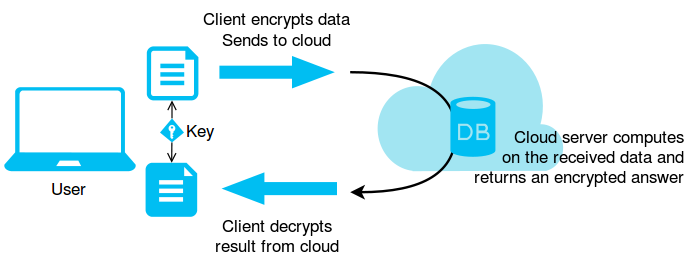
\includegraphics[scale=0.5]{he.png}
	\caption{Illustration of a homomorphic system where data is encrypted at the client, sent to the server which performs computation on the encrypted data and returns an encrypted result which is decrypted by the client.}
	\label{fig:he_ill}
\end{figure}

Regular \gls{pke} schemes consists of three algorithms, namely a key generation algorithm (\texttt{KeyGen}), an encryption algorithm (\texttt{Enc}) and a decryption algorithm (\texttt{Dec}). \gls{he} schemes adds another algorithm to the toolbox, an evaluation algorithm (\texttt{Eval}).  Assume a well formed public key $pk$, a boolean circuit $C$ and a set of ciphertexts $c_1, ..., c_l$ which are encryptions of $m_1, ..., m_l$ respectively. Then \texttt{Eval} outputs a ciphertext $c$ which encrypted under $pk$ such that $Dec_{sk}(c) = C(m_1, ..., m_l)$ for some secret key $sk$ \cite{damgaard2012secure}.


For \gls{phe} schemes, $Eval$ will be associated to a set of permitted functions $f$ (or circuits). These are functions that the algorithm can handle, and which guarantee a meaningful result when executed. These functions can be expressed as boolean circuits consisting of logical gates such as AND, OR and NOT. Gentry \cite{Gentry_computing_arb_func_enc_data} presented a homomorphic encryption scheme consisting of three functions; addition ($Add_{\epsilon}$), subtraction ($Sub_{\epsilon}$) and multiplication ($Mult_{\epsilon}$). When performing homomorphic operations using functions from $f$, an N-bit noise is generated and added to the encrypted ciphertext, making the relation between the encrypted result and its corresponding plaintext weaker. By performing multiple operations on the ciphertexts, the noise grows larger. Problems arise when the noisy part gets too large, as the decryption algorithm might not be able to decrypt in a reliable way in order to obtain the correct result.

\section{Fully Homomorphic Encryption}

\Gls{fhe}, which has no restrictions to what types of operations that can be performed on the encrypted data, was first suggested in 1978 by Rivest, Adleman, and Dertouzos \cite{rivest1978data}. At this point in time, researchers did not have any secure scheme for using these ideas. More importantly, there were not many use cases driving the need of such schemes. It has therefore been a slightly displaced and forgotten grail until 2009,
when Gentry presented the first \gls{fhe} scheme based on lattices \cite{Gentry_first_lattices}, and a year later another scheme using a \emph{bootstrappable} approach \citep{Gentry_computing_arb_func_enc_data}. Nearly all modern \gls{fhe} schemes are based on this bootstrappable concept using Gentry's blueprints. 

As mentioned in the section above, a homomorphic operation creates noise when executed. Multiple operations adds more noise which may change the decrypted result beyond the recognizable. But what if we had a scheme that was able to reduce the noise generated by such operations? Boostrapping involves encrypting the secret key $sk$ under its corresponding public key $pk$ and added to a modified encryption algorithm, $Recrypt(pk_{i+1}, D_{\epsilon}, \overline{sk_i}, c_i)$. This basically enables the algorithm to decrypt the ciphertext $c_i$ taken as input internally while being encrypted under the new public key $pk_{i+1}$. $Recrypt$ returns a \emph{freshly} created ciphertext $c_{i+1}$ which is less noise than the original $c_1$ ciphertext to continue to perform homomorphic operations on.

Equation \ref{enc_m} encrypts the message $m$ under the public key $pk_1$ as most asymmetric encryption schemes does, in order to obtain the ciphertext $c_1$. So far, nothing we have not seen before. Now, the secret key $sk_1$ from the public-key-pair $(pk_1,sk_1)$ is encrypted using a new, fresh public-key pair $(pk_2, sk_2)$ as seen in Equation \ref{enc_sk}. By doing so, the algorithm enables $Eval$ to later on decrypt $c_1$ using $sk_1$ while under the encryption of $pk_2$.

\begin{equation}
\label{enc_m}
c_1 = Enc(pk_1, m)
\end{equation}
\begin{equation}
\label{enc_sk}
\overline{sk_1} = Enc(pk_2, sk_1)
\end{equation}


Bootstrapping works recursively, so for the algorithm to be able to decrypt the $c_1$ in the next iteration, it needs to be encrypted under the new public key $pk_2$ as seen in Equation \ref{enc_c_1}. In Equation \ref{eval_c1_pk2}, a new and fresh ciphertext is produced by the $Eval$ algorithm, which uses $pk_2$ to encrypt the noisy ciphertext $c_1$, and D to decrypt it $c_1$ using its corresponding $sk_1$ inside $Eval$. By doing this, the noise of the ciphertext is reduced, while still being encrypted - Now under the public key $pk_2$. Figure \ref{recrypt_function} shows the process of the $Recrypt$ algorithm.

%% Dette er piss. 


\begin{equation}
\label{enc_c_1}
\overline{c_1} = Enc(pk_2, c_1)
\end{equation}
\begin{equation}
\label{eval_c1_pk2}
c_1' = Eval(pk_2, D_{\epsilon}, \overline{sk_1}, \overline{c_1})
\end{equation}


\begin{figure}[h]
	\centering
	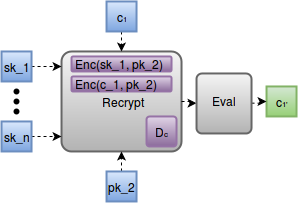
\includegraphics[scale=0.8]{bootstrapp.png}
	\caption{Illustration of the Recrypt algorithm, which refreshes the ciphertext $c_1$ encrypted under the new public key $p_2$.}
	\label{recrypt_function}
\end{figure}



When allowing the encryption function to handle its own decryption function at the same time, Gentry showed that the noise added by the homomorphic operations was less than the noise removed by the additional decryption \cite{Gentry_computing_arb_func_enc_data}, and the breakthrough was made in hunt for a fully homomorphic encryption scheme. While Gentry's system is great in theory, it has been shown that creating \gls{fhe} schemes is hard in practice. However, some other cryptographic schemes holds different types of homomorphic properties which when combined can provide different homomorphic operations. Addition is, for example, a homomorphic property of the Pailler cryptosystem \citep{Paillier}. Pailler is originally a trapdoor mechanism based on the Composite Residuosity Class Problem which conveniently has the cryptographic property such that \[ENC_k(x) * ENC_k(y) = ENC_k(x + y)\]

Another practical cryptosystem providing a similar property, is the ElGamal cryptosystem \cite{elgamal}. Along with being an asymmetric cryptosystem , it has the cryptographic property shown below, which enables it to perform homomorphic multiplications.  \[ENC_k(x) * ENC_k(y) = ENC(x * y)\]




\chapter{Overview of CryptDB}
\label{chp:overview_cryptDB}

This chapter covers the overview of CryptDB, starting with the system architecture, followed by its different encryption mechanisms and encryption layer adjustments. Along with the investigation, a small application will be introduced and used as an example to help the reader in understanding the practical and impractical usages of CryptDB.

\section{System Architecture}
\label{sec:sysarc}

CryptDB's architecture (Figure \ref{cryptdb_plain}) is divided into two pieces, a proxy server and a database server. The proxy server is an intermediate server placed between the application server (used by the application to manage key set-up and interacting with clients) and the database server. The proxy server's purpose is to intercept queries going from the application to the database and anonymize the information of the query, as well as decrypting results going from the database server to the user's application. By doing so, it eliminates the possibility of eavesdropping attackers to obtain any sensible information. %Kommentere at Microsoft hevder å ha brukt freq attack her.

\begin{figure}[H]
	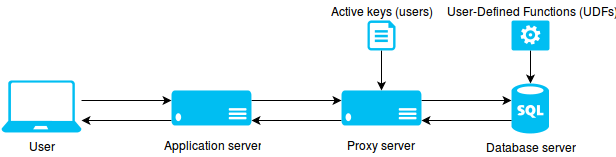
\includegraphics[scale=0.58]{CryptDB_Plain.png}
	\caption{System architecture of CryptDB interacting with a client application}
	\label{cryptdb_plain}
\end{figure}

Another vital part of the proxy server's domain is to issue queries to the database that adjusts the encryption layer (or onion layer) of the data items(s) that the user has issued a query on, which will be discussed in section \ref{adjust_enc_level}. The last responsibility of the proxy server is to keep track of the users that are currently logged in using a table of active keys. In addition to keeping the list of active keys, the proxy server also keeps an embedded database with the schemes of the encrypted tables in the database. By storing this, the proxy server keeps a continuous picture of the encryption layer for each column, which is used for adjusting the encryption level (or layer) for a column in order to allow certain types of functionality.

The authors \citep{CryptDB_Main_Paper} have implemented CryptDB both with MySQL and PostgreSQL database management systems. CryptDB requires no modifying of the database system, other than adding a set of \Gls{udf}. \Gls{udf} in CryptDB allows the database to perform cryptographic operations on the encrypted data, as well as adjust the encryption level of different columns.

CryptDB has two operational modes, or principals. One for applications consisting of only one user, and another for multi-user applications. Application keys consists of both a symmetric key rooted in the users application password and a public-key pair. When logging in, the proxy derives encryption keys with the user's password as the root. These keys are used for accessing the data items that are accessible to that particular user and to encrypt new items. When the user logs out, the keys are deleted from the proxy server.



\section{SQL-Aware Encryption and the Onion Scheme}
\label{sec:sqlaware}

\begin{wrapfigure}[19]{r}[1pt]{4cm}
\centering
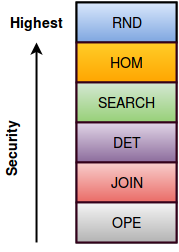
\includegraphics[width=\linewidth]{encstack/enc_stack_ope.png}
\caption{Ordering of the different encryption layers based on their security}
\label{fig:enc_stack}
\end{wrapfigure}

CryptDB uses an encryption scheme called \emph{SQL-aware encryption} or \textit{onion encryption}. Basically, this is a collection of different encryption schemes, each providing different levels of security and computations to be executed. Data items stored using CryptDB are encrypted multiple times using these different schemes, or layers, of encryption. The result is a onion-like structure where the outer layers provide maximum security and low functionality, while the inner layers provide less security, but more functionality. Figure \ref{fig:enc_stack} shows the ordering of the different layers from most secure to least secure. Each layer will be explained throughout this section.

As a scenario in order to describe the different operations and situations in CryptDB, assume a simple employee application with a table structure and some example records as shown in Table \ref{demoapp_table}. Our application is created in order to provide some insight in the salary distribution within our firm, with respect to age, number of years within the firm and employment division. EmplNum is the number associated with the employee in other systems and applications, and SSN is the Social Security Number of the employee used for creating pay checks and similar operations.

\begin{table}[H]
\centering
\begin{tabular}{| r | r | l | r | r | r | l |}
\hline
  Id & EmplNum & Name & SSN & Age & Salary & Division \\
  int & int & varchar(255) & varchar(255) & int & int & varchar(255) \\
 \hline \hline
 1 & 42 & Alice & 24127312345 & 42 & 440000 & Marketing \\
 2 & 1 & Bob & 17054623456 & 69 & 850000 & Management \\
 3 & 1337 & Charlie & 31129134567 & 23 & 390000 & Engineering \\
 4 & 123 & Donna & 11117945678 & 36 & 510000 & Management \\
 \hline

\end{tabular}
\caption{Employee table for a simple employee application with example records}
\label{demoapp_table}
\end{table}



\subsection{Random}

\Gls{random_onion} is the highest security level in CryptDB and provides the maximum security found in encryption scheme. It uses a strong block cipher such as Blowfish or \Gls{aes} in \Gls{cbc_mode} mode and a random initialization vector (IV) to ensure that the block cipher is probabilistic \citep{CryptDB_Main_Paper}. \Gls{random_onion}, being the maximum security level provided, does not allow any computation to be done on the encrypted data. In other terms, this level is a natural choice for sensitive data that are only meant to be read. When a block cipher is probabilistic, it has properties such that when encrypting the same message $m_1$ multiple times, the resulting ciphertexts are unequal. 

For example, given two encryptions of the same plaintext $c_1 = E_k(m_1)$ and $c_2 = E_k(m_1)$, the resulting ciphertexts are $c_1$ and $c_2$ such that $c_1 \neq c_2$. Operations supported by this scheme are \verb!SELECT!, \verb!UPDATE!, \verb!DELETE! and \verb!INSERT!. It also supports altering an existing table by removing or adding columns using the \verb!ALTER! statement. In our sample application, the SSN would be the most natural thing to stay encrypted under \gls{random_onion} at all times, as there are not many natural operation to perform on such numbers. However, the other columns are not likely to be encrypted under \gls{random_onion} as it is likely that the application would want to perform some operations which demands a lower encryption level. As for an example, take the perhaps most natural query at this encryption level, the \verb!INSERT! statement

\begin{verbatim}
INSERT INTO employee_table
VALUES('', 5, 'Eric', '29026056789', 55, 680000, 'Engineering');
\end{verbatim}

\noindent
which adds a record in the database containing Eric's information. When it comes to \verb!SELECT!, \verb!DELETE! and \verb!UPDATE!, it only supports regular queries without the \verb!WHERE! clauses and similar statements:

\begin{verbatim}
SELECT * FROM employee_table;

UPDATE employee_table SET salary = 0;

DELETE FROM employee_table;
\end{verbatim}



\subsection{Homomorphic Encryption}

Another vital part of \Gls{sql} is the ability to perform addition and multiplication. For CryptDB to be able to perform these operations, it utilizes a \Gls{hom_onion} scheme. As previously described, homomorphic encryption is a technique that enables computation on encrypted data without decrypting it first. CryptDB uses Pailler multiplication \cite{Paillier} for enabling summation operations. If our application is in need for finding out the total sum of the salaries within the firm, we do something like this

\begin{verbatim}
SELECT SUM(Salary)
FROM employee_table;
\end{verbatim}

\noindent
Or extracting the total salary for each division by using the \verb!GROUP BY! clause

\begin{verbatim}
SELECT Division, SUM(Salary)
FROM employee_table
GROUP BY Division;
\end{verbatim}

\noindent
Multiplication was not initially implemented, but has been implemented in some versions of CryptDB by an outside team using the El Gamal cryptosystem \cite{cryptdb_guidelines}. 



\subsection{Search}

In order to perform search for words in the encrypted texts, CryptDB has a scheme called SEARCH. This was an implementation of the cryptographic protocol suggested by Song et al. making it almost as secure as the \gls{random_onion} scheme \citep{CryptDB_Main_Paper}. The main idea is to split a text encrypted with SEARCH into individual keywords on a given delimiter specified by the application developer. Removal of duplicate keywords and randomly permute them are also added to enhance the security. When executing a search, the server would be given an encrypted token of the keyword, and would retrieve encrypted values matching the token. Originally, SEARCH could perform \texttt{LIKE} operations as other database systems, but in the most recent version of CryptDB's software it has been deprecated. 

% SKRIVE OM AT DET ER ISH SOM DET


\subsection{Deterministic}
\label{sec:det}

As \Gls{random_onion} allows no computation to be done on the encrypted data and \gls{hom_onion} only allows addition, the next layer brings some more functionality to the toolbox. \Gls{deterministic_onion} is an encryption scheme enabling the application to perform standard SQL operations such as equality checks, distinct, group by and count. By allowing these sorts of computation, the application leaks information to an adversary. In particular, it leaks which ciphertexts that decrypts to the same plaintext value. Following the previous example; if the scheme encrypted the message $m_1$ two times, the resulting ciphertexts $c_1$ and $c_2$ are such that $c_1 = c_2$. For our sample application, \Gls{deterministic_onion} would be the scheme used when allowing operations such as \verb!GROUP BY!, \verb!DISTINCT! and \verb!COUNT!. Continuing with our sample application, we now want to find out what types of departments that exists in our table

\begin{verbatim}
SELECT DISTINCT Division
FROM employee_table;
\end{verbatim}
\noindent
which returns \verb!'Engineering'!, \verb!'Marketing'! and \verb!'Management'!. As described, a deterministic scheme encrypts the same plaintext to the same ciphertext every time. By taking advantage of this, CryptDB is capable of iterating over the encrypted data and return a distinct selection of the different ciphertexts observed. At the \gls{deterministic_onion} layer the \verb!WHERE! clause is also supported when running equality checks. An example usage is the query below, where the name, age and salary of all employees from the management division are returned

\begin{verbatim}
SELECT Name, Age, Salary
FROM employee_table
WHERE Division = 'Management';
\end{verbatim}

For the encryption, DET uses a strong block ciphers, and either with 64-bit or 128-bit block size. If a value is larger than 128-bits, it leaks  prefix equality when used with AES \citep{CryptDB_Main_Paper}. In order to cope with leaking prefix equality, the authors have designed their own version of the CMC mode.



\subsection{Order-Preserving Encoding}
\label{sec:ope}

Since \Gls{sql} also allows the user to compute on order relations between items, CryptDB introduces an \Gls{ope_onion} scheme \citep{CryptDB_Main_Paper}. This scheme is based on a requirement where the sort order of the ciphertext matches the sort-order of the corresponding decrypted plaintexts. It also requires that the scheme reveals no other information about the plaintexts, other than the respective order. For example, if a value $x \ge y$ then the corresponding encryption would be such that $Enc(x) \ge Enc(y)$. In \Gls{sql}, such an operation is used for order comparison, which are range checks, ranking, sorting, and extracting minimum and maximum values. 

CryptDB uses a modified version the scheme proposed by Boldyreva et. al \citep{ope_cryptdb} as their OPE scheme, which is a random order-preserving injective function. An injective function is a one-to-one random mapping function that preserves the order of the elements. Since queries related to order consists of retrieving items between two values, or ranges related to one particular value, the encrypted values can be stored as binary trees at the server, ensuring logarithmic run-time \cite{ope_cryptdb}.


% Fjerne figuren?

\begin{figure}[h]
	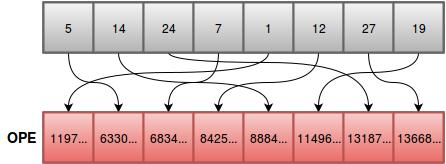
\includegraphics[scale=0.7]{one-to-one.png}
	\caption{Order-preserving encryption of a set of integer values}
	\label{fig:ope_function}
\end{figure}

Figure \ref{fig:ope_function} shows the order-preserving encryption of a set of integers, where no information is leaked, except for the order of the ciphertexts. When searching for the persons in our imaginary firm that has a yearly salary over 500 000, the query uses the \verb!WHERE! clause and then performs an order check where it navigates down the binary three for items that has a salary larger than the requested value.

\begin{verbatim}
SELECT Name, Salary
FROM employee_table
WHERE Salary > 500000;
\end{verbatim}

Popa et al. have also proposed their own OPE scheme to go with CryptDB \cite{CryptDB_OPE_Encoding}, but due to other priorities, this scheme was never actually implemented into CryptDB's software.



\subsection{Equality Join and Order-Preserving Join}

When it comes to joining columns, two cases are supported in CryptDB. The first is the regular equality join (EQ-JOIN) between two columns, and the other is range joins (OPE-JOIN) which involves order relation checks. Ideally, the proxy server should know in advance which columns that should be allowed to be joined in order to encrypt these column with the same key. Because of the key-chaining approach where each data item is encrypted with a new key, CryptDB is in need of a separate encryption scheme in order to compute joins in a safe manner.

The authors \citep{CryptDB_Main_Paper} introduces a new cryptographic primitive for equality joins, \gls{join_adj}, which is a deterministic function. The idea is to let the proxy server adjust the encryption keys of columns in real-time, based on the observed query. By using this approach, CryptDB avoids the database server to compute joins on its own as attempt to learn about relations between different tables and columns. When a join query is observed at the proxy, it sends an adjusted key to the database server enabling it to adjust the values in one of the two affected columns. When an adjustment has been done, the columns share the key until the proxy server issues a new adjustment key to either one of the columns.

The second case is the order-preserving join, which depends on the \gls{ope_onion} scheme previously described. The binary tree structure of the scheme makes in infeasible to use the same approach as EQ-JOIN. Therefore, CryptDB has a requirement that columns where such joins is applicable have to be declared by the application in beforehand and encrypted under the same key. If this measure has not been addressed, CryptDB will simply encrypt all columns with the same key.

\begin{table}[H]
\centering
\begin{tabular}{| r | r | l | r | l | r |}
\hline
  Id & EmplNum & University & Graduated & Degree & AdjustedGPA* \\
  int & int & varchar(255) & int & varchar(255) & int \\
 \hline \hline
 1 & 42 & HiST & 1993 & B.Sc. & 319 \\
 2 & 1 & NTNU & 1971 & M.Sc. & 305 \\
 3 & 1337 & UiO & 2015 & M.Sc & 287 \\
 4 & 123 & NHH & 2009 & MBA & 392 \\
 \hline
\end{tabular}
\caption{Educational table for the employee application. \emph{*Because of no support for floating values, the GPA is multiplied by 100 and rounded down.}}
\label{tab:demoapp_education}
\end{table}

Assume that along with the table of employees, there is also a table holding the employees educational information as seen in Table \ref{tab:demoapp_education}. By performing a join between our two tables on the shared employee number EmplNum, it is possible to extract information from the two combined tables.

\begin{verbatim}
SELECT Name, Division, University, Graduated
FROM employee_table t1
JOIN employee_education t2
ON t1.EmplNum = t2.EmplNum;
\end{verbatim}

\subsection{Wrapping the Layers}

These different layers are wrapped into four different classes or \emph{onions}, namely \texttt{EQ}(Equality checks), \texttt{ORD}(Order relations), \texttt{SEARCH}(Searching) and \texttt{ADD}(Addition) as shown in Figure \ref{cryptdb_onions}. Each onion has a special purpose in means of supporting certain operations, and every data item is encrypted each of the different onions using the different layers. However, the application does not necessary maintain all of onions. There is, for example, no need for maintaining the ADD-onion if the data item is a string.

\begin{figure}[H]
	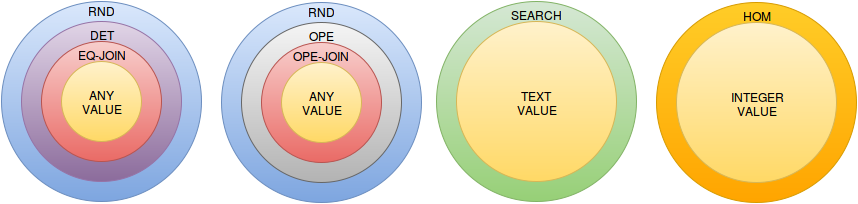
\includegraphics[scale=0.42]{Onions.png}
	\caption{Overview of the structure of the SQL-aware Encryption Scheme. From left: The EQ-onion, ORD-onion, SEARCH-onion and ADD-onion}
	\label{cryptdb_onions}
\end{figure}


\section{Adjusting the Encryption Level Based on the Query}
\label{adjust_enc_level}

Okay, so there is an encapsulation of different encryptions for each data item, and our ideal scenario is that our data is encrypted at the highest, feasible level at all times.  But how is the system supposed to perform a range check if the utmost layer is the \gls{random_onion} which does not support any functionality at all?

CryptDB solves this particular case gracefully by having the proxy server observe incoming queries in real-time. After observing a query, it checks its embedded table holding the encryption level of the all columns whether or not the current encryption level of the inflicted columns are supporting the query. For example in our sample application, the user has issued the query 
\begin{verbatim}
SELECT *
	FROM employee_table
	WHERE salary > 5000000;
\end{verbatim}

Have in mind that all data items at this point is encrypted with \gls{random_onion} as the utmost layer. What the proxy does, is that before sending the rewritten query to the database server, it sends an \verb!UPDATE! query first. This query orders the database server to remove the outer encryption level of the ORD-onion to match the \gls{ope_onion} layer, before it sends the rewritten query. Figure \ref{ope_layer_adjustment} illustrates how the proxy server observes the query, and issues the \verb!UPDATE!. \verb!SET! is used to change the current encryption level of the ORD-onion, and \verb!cryptdb_decrypt_int_sem! is the name of the UDF that the server will use to adjust the encryption layer to  support the query. The curious string \verb!'???]???G??+?,?#'! is the encrypted key which the server will use along with the UDF.

\begin{figure}[h]
	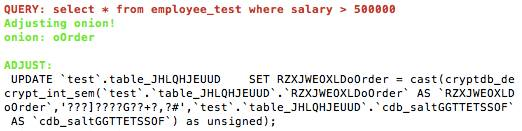
\includegraphics[scale=0.7]{terminal/adjustOnionLayer.jpg}
	\caption{Encryption layer adjustment performed by proxy server upon receiving a query. (Is the figure too small/hard to read?. Adjust colors?)}
	\label{ope_layer_adjustment}
\end{figure}

After performing the encryption layer adjustment, the proxy rewrites the query as shown in Figure \ref{rewritten_query}. As described, each of the columns are anonymized upon the creation of a table. The proxy server keeps table schemes in order to substitute the different parts of the query so it matches the encrypted columns in the database. For the record, 'test' is the name of the current database.  

\begin{figure}[h]
	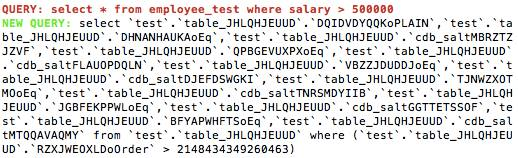
\includegraphics[scale=0.7]{terminal/executeQuery.jpg}
	\caption{Rewritten query to be sent to server after encryption level adjustment. (Is the figure too small/hard to read?. Adjust colors?)}
	\label{rewritten_query}
\end{figure}

When a layer has been stripped off, it does not automatically get re-encrypted unless the developer has specified such actions. For example, if an irregular query forces the encryption level lower than necessary. For applications running in single-mode, the encryption layers will over time be in a stable state supporting the relevant queries. But, for multi-mode applications, the developer decides the functionality, hence the types of queries that the application can produce. Therefore, it is possible to start application at the correct layers based on the wanted functionality, and the proxy does not perform any encryption level adjustment at all.



\section{Security}

In section \ref{sec:sysarc}, two different modes for using CryptDB was mentioned. For applications built for one particular user, the single-user mode of CryptDB is used. Example of applications where such a mode would be useful is when creating a personal diary application or a contact list application. When building applications consisting of users and interaction between users, the developer needs to use the multi-user mode.

\subsection{Single-user Mode}
If an application is created with a single user in mind, then it should be running in the single-user mode where the keys are derived from one secret master key which is rooted in the user's password. By running in this particular mode, the user has access to all data encrypted through the proxy server. When running is this mode, the proxy server and the application are considered to be trusted. The database server however, is considered to be untrusted and subject to the snooping of a curious database administrator owning the server system hosting the database. As of the most recent versions of the CryptDB software, only the single-user mode is supported, which has been used to create a small demo application described in Chapter \ref{chp:software}.

\subsection{Multi-user Mode}
Picture a simple online discussion forum, where users can interact by posting messages to discussion boards or sending each other private messages. As described in Section \ref{chp:database_Security}, database applications are in need of access control in order to restrict access to certain tables based on the user's credentials, hence the need for declaring user entities as well as different groups. But how can a user read messages on the discussion board if they are encrypted by another user's key? What about private messages, with suffers from the same case, as they will be encrypted with the sender's key? CryptDB solves these cases by letting developers use annotations in their schemas.

Table \ref{annotations} shows a basic use of such annotations. \verb!PRINCTYPE! is used to annotate external users, which are authenticated through the access control by providing their password, and internal users, which are entities inside the database. \verb!ENC_FOR! is used to indicate which columns that consist sensitive data, and in the next column CryptDB needs to store which principals that should have access to the sensitive column. Okay, so we have access to the column, but how can we decrypt something encrypted with someone else's keys?

\begin{table}[H]
\begin{Verbatim}[frame=single]
PRINCTYPE physical_user EXTERNAL;
PRINCTYPE user, msg;

CREATE TABLE privmsgs (
	msgid integer,
	subject varchar(255)	ENC_FOR (msgid msg),
	msgtext text		ENC_FOR (msgid msg) );

CREATE TABLE privmsgs_to (
	msgid integer,
	recvid integer,
	sendid integer,
	(sendid user) SPEAKS_FOR (msgid msg),
	(recvid user) SPEAKS_FOR (msgid msg) ); 
\end{Verbatim}
\caption{Use of policy annotations when creating multi-user applications}
\label{annotations}
\end{table}

CryptDB chains encryption keys used to encrypt columns or data items to the root key, which is the user's password. The \verb!SPEAKS_FOR! annotation gives a principal access to all the keys that the principal it speaks for has access to. For example in Table \ref{annotations}, both the user sending the private message and the user receiving it, speaks for the principal type \verb!msg! and thereby has access to all the keys of the \verb!msg! entity. This basically means that the secret key of the message is encrypted two times, one time with the sender's key and one time with the receiver's key.

Consider this case: Alice wants to send a private message to Bob, which means that the private message needs to be encrypted two times using both Alice and Bob's secret keys. Keys of users who are logged in are kept in a table at the proxy server, but what happens when the proxy server needs to encrypt something with a key which at the time is inaccessible? The keys that are used by a principal to encrypt consists of both a symmetric key and a public-private-key pair. When both parties are logged in, the proxy uses their symmetric keys to encrypt the message. If Bob is currently logged out, the message is encrypted using his public key so that he can decrypt it using the corresponding private key when he logs in.

As previously mentioned, the current version of CryptDB has only the option of developing single-mode applications. One may react to the fact that the developers has stopped maintaining such a useful way of developing applications with multiple user's and interaction between users. However, Mylar \cite{mylar_homepage} is the creators of CryptDB's new project. Mylar addresses the threat of the insecure proxy server being compromised by an attacker, and how to protect the confidentiality of the users' data in such events. During an attack on the proxy server in CryptDB, the only parties that are compromised are those who are currently logged in, where their keys are stored at the proxy server.


\subsection{Securing Applications When Using CryptDB}
\label{sec:sensitive}

Another importance related to annotations is the use of the \verb!SENSITIVE! annotation. By labelling columns as sensitive, CryptDB provides strong security guarantees of the data stored in the affected columns and also semantic security \cite{popa_thesis}. When a column is marked as sensitive, the only encryption schemes that are allowed are \gls{random_onion}, \gls{hom_onion}, SEARCH and, if the column has the \verb!UNIQUE! constraint from \gls{sql}, \gls{deterministic_onion}. The reason for enabling the \gls{deterministic_onion} scheme under a constraint of the data being unique, is as there are no equal plaintexts, there will be no equal ciphertexts, and the scheme leaks no information about the encrypted data.

%When encrypted under these schemes, the available set of operations are limited compared to CryptDB's full set of operations. However,

\section{Limitations}

\gls{fhe} is nowhere near being practical yet, but CryptDB tries it best to be a somewhat practical \gls{he} scheme allowing a set of operations that they claim to be enough to support 99.5\% of all queries observed in a \gls{sql} trace from a production MySQL server \citep{CryptDB_Main_Paper}. Although, there are multiple fairly trivial data types that CryptDB does not support.

For example, all fixed-point types and floating-point types are not supported, meaning that computing on decimal values are difficult for the application to perform. In Table \ref{tab:demoapp_education}, our GPA-column, where the most natural data type would be decimal, has been adjusted to integer by the application. One way to cope with the limitations, is to let the developer be responsible to transform a data type that is not supported into a supported one, and handle the inverse transformation  upon receiving an encrypted result. Another option is to let CryptDB exclusively store such values as text with \gls{random_onion} or \gls{deterministic_onion} encryption, and let client perform operations on such data types. As you probably understand, the last option is not desirable, as it is quite the opposite the goal when using such schemes as CryptDB. 

Another data type that is not supported is those related to date and time, namely Timestamp, Date, Time, DateTime, Year and NewDate. In other terms, if your application needs to encrypt dates and at the same time be able to compute on them, you are in bad luck. The authors suggestion is to encrypt each part of a data in separate columns, and perform the computations on those columns instead of a composite date column. While being a rather complicated approach, it works surprisingly well for our demo application. Assume that we add some more columns to Table \ref{demoapp_table} with the precise date of birth in stead of age as seen in Table \ref{tab:empl_tab_mod}.

\begin{table}[H]
\centering
\begin{tabular}{| c | r | r | r | c |}
\hline
  ... & Day & Month & Year & ... \\
  ... & int & int & int & ... \\
 \hline \hline
 ... & 24 & 12 & 1973  & ... \\
 ... & 17 & 05 & 1946 & ... \\
 ... & 31 & 12 & 1991 & ... \\
 ... & 11 & 11 & 1979  & ... \\
 \hline
\end{tabular}
\caption{Additional columns to the employee table with date properties stored in separate columns}
\label{tab:empl_tab_mod}
\end{table}

Consider 17th of May 1980 as our test date, and that we want all employees born after the test date. In a regular database system supporting date related data types, our query would be something like this on a concatenated date of birth column

\begin{verbatim}
SELECT Name, date_of_birth
FROM employee_table
WHERE date_of_birth > '17/5/1980'
ORDER BY date_of_birth ASC;
\end{verbatim}

As for CryptDB where such queries do not return anything meaningful, we need to modify our approach as seen below

\begin{verbatim}
SELECT Name, Day, Month, Year
FROM employee_table
WHERE (year = 1980 and month = 5 and day > 17)
OR (year = 1980 and month > 5)
OR (year > 1980)
ORDER BY year ASC, month ASC, day ASC;
\end{verbatim}

Queries are also subject to some constraints. In \gls{sql}, users are also allowed to use \emph{subqueries} or \emph{nested queries}, which is an \gls{sql} query embedded inside another query using the \verb!WHERE! clause. Such subqueries are used by the main query to retrieve data that will be used as a condition in order to further restrict its result. If we now want to retrieve salaries for employees' graduating after 1980, a regular \gls{sql} query would be something like this

\begin{verbatim}
SELECT Name, Salary
FROM employee_table
WHERE EmplNum IN
    (SELECT EmplNum
    FROM employee_education
    WHERE graduated > 1980);
\end{verbatim}

In CryptDB, such queries are infeasible, which leaves us with two options. Option one is to perform a join instead using subqueries. While this may solve our problem in this particular situation, it does not necessary work in all situations and may create duplicated rows in the result. Option two is to let the application execute the operation as two separate queries and store the result of the first query as an intermediate value used in the second query.

\begin{verbatim}
temp_result :=
    SELECT EmplNum
    FROM employee_education
    WHERE graduated > 1980;

SELECT Name, Salary
FROM employee_table 
WHERE EmplNum IN (temp_result);
\end{verbatim}


Along with complicating tables and adding overhead to the database, such limitations also puts the responsibility of the developer to add software code on the application server or client side. For larger applications and complex operations, such actions are not necessary feasible and hence an limitation to the use of CryptDB as a database system.

\chapter{Attacking CryptDB}
\label{chp:attacks}

In this chapter, a few known attacks on CryptDB will be presented along with the discussion around...

\section{Tampering with CryptDB}

Akin and Sunar \cite{akin_2014} introduces an attack approach where a malicious database administrator targets web applications running in multi-user mode. More specific, software developed using the popular open-source software phpBB \cite{phpBB} where highly customisable forums can be created. By creating a fake user through the web application, and at the same time being able to observe queries arriving at the database server, a malicious database administrator is able to attack CryptDB.

When creating tables in CryptDB, the order of the columns are preserved. By combining this information with the publicly available source code from phpBB, the attacker is able to understand the encrypted schema of the user table. When creating the fake user and logging in, the administrator can observe in the database the login attempt, and also determine the fake user's row id. By trying to log in with someone else's user-name (and obvious failing), the administrator is able to locate a specific user in the encrypted table. Now the malicious administrator can start to tamper with the database.

By copying any user's encrypted information directly into the fake user's corresponding fields, the attacker may be able to obtain encrypted information without necessary breaking the encryption. Another possibility is for the database manager to overwrite the password of every user with the encrypted version of the fake user's password. The consequence of this scenario is a database manager that can log into the application with every user.

% Kan ta med det å joine to kolonner på samme id for å intersekte to sykehusbesøk.

It is clearly stated that CryptDB does not provide any other security guarantees except for data confidentiality \cite{CryptDB_Main_Paper}. As this attack clearly targets data integrity, it is not necessary CryptDB's a weakness in the software itself. However, it gives a good example on how providing data confidentiality is not enough in order to secure a database system. Data integrity should be provided for both the encrypted data as well as the queries observed at the database.

\section{Microsoft Research and their Frequency Analysis}

In September 2015, a Microsoft Research team released a paper stating that they had successfully broken the \gls{ope_onion} and the \gls{deterministic_onion} encryption schemes of CryptDB \cite{microsoft_cryptdb}. They did so by using one of the oldest trick in a crypt analyst's book; frequency analysis.

\begin{wrapfigure}[13]{r}[1pt]{5.2cm}
\centering
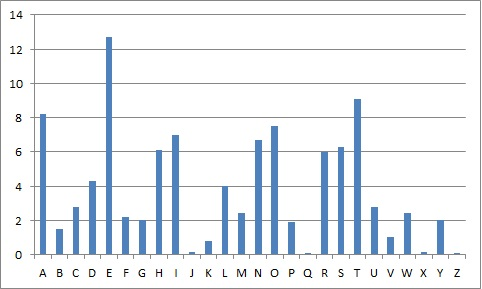
\includegraphics[scale=0.4]{letterfreq.jpg}
\caption{Bar chart of the letter frequency observed in the English language}
\label{fig:letter_freq}
\end{wrapfigure}
Frequency analysis is to exploit the fact that in most spoken languages, some characters and combinations of characters are more common than others. In the English alphabet, E, T, A and O are the most regular characters, while J, Z, Q and X are considered to be rare. As described in \ref{sec:det} and \ref{sec:ope}, the DET and OPE schemes are deterministic and therefore encrypts the same plaintext to the same ciphertext. \gls{ope_onion} also reveals the order between the ciphertexts. Because of this, an attacker with access to the ciphertexts is able to compute a histogram of the observed frequencies in the encrypted data. By comparing the histogram to a similar histogram of frequencies computed from closely related plaintext data, the attacker is able to determine which ciphertext characters corresponds to which plaintext characters with fairly large advantage.

% ???
As described in section \ref{sec:sqlaware}, in order for an application to be able to execute equality checks or order comparison, columns need to be encrypted with DET or OPE respectively. 




From an encrypted test database containing health records from multiple hospitals in the United States, Naveed, Kamara and Wright claimed to successfully have recovered 80\% of OPE-encrypted ciphertexts from 95\% of hospitals, and 60\% of DET-encrypted ciphertexts from 60\% of hospitals \cite{microsoft_cryptdb}. Their concrete attacks was a regular frequency analysis for attacking DET-encrypted columns along with a new attack called \emph{P-Optimization}. For decrypting OPE-encrypted columns, they used a regular sorting attack and a new cumulative sorting attack.

\subsection{Frequency Analysis on DET-encrypted Columns}

For decrypting DET-encrypted columns, frequency analysis was used where the $i$th most frequent element of an encrypted column $c$ was assigned to the $i$th most frequent element in an auxiliary dataset built with similar structured data. In addition to performing a plain frequency analysis, the researchs also presented a new attack called \emph{P-Optimization}. Instead of ordering frequencies from most frequent to less frequent, they find an allocation of ciphertext-plaintext pairs that minimizes the overall difference between the histogram computed by the frequency analysis and the auxiliary one. Finding the allocation that minimizes the difference in the histograms is formulated as \gls{lsap}, and can be solved by using a linear programming solver \cite{microsoft_cryptdb}.

For DET-encrypted columns, these attacks recovered the mortality risk and whether a patient lost its life while under hospital care for 100\% of the data items in 99\% and 100\% of the hospitals respectively. They also recovered 100\% of the data items in the column storing the severity of a disease for 51\% of the hospitals. Additionally to these columns, they also show that it is possible to decrypt some of the information related to race, sex, admission type, primary payer and major diagnostic category \cite{microsoft_cryptdb}.

\subsection{Sorting Attack on OPE-encrypted Columns}

When attacking columns encrypted using the OPE scheme, Microsoft Research used two approaches. The first approach was to use a sorting attack given that all of the columns where \emph{dense}. By dense, they mean that both the encrypted column and the equivalent column in the auxiliary dataset contains every element from the plaintext space. By sorting both values from the encrypted column and the auxiliary dataset and map the values based on rank, the attack is able to decrypt 100\% of the encrypted column. However, if the column does not contain all the possible plaintext from the plaintext space, the methodology has to be modified.

Cumulative attack for low-density columns is an approach where the attacker does not only leverage the scheme leaking the frequency of the ciphertexts, but also the relative ordering of the ciphertexts. If a ciphertext $c$ is greater than 90\% of the ciphertexts in the encrypted column, then it should be matched against values that are greater than 90\% of the elements in the plaintext space. By combing a \gls{cdf} and frequency analysis, and using an \gls{lsap} solver to find the most optimal pairing of ciphertexts and corresponding plaintexts, Microsoft Research was able to recover more than 80\% of encrypted data from 95\% of the hospitals \cite{microsoft_cryptdb}.

\subsection{CryptDB Developers Answer Microsoft Research}

In response to Microsoft Research's paper, the developers of CryptDB has presented a paper containing guidelines \cite{cryptdb_guidelines} on how to safely use CryptDB and remarks on where they claim Microsoft Research has used CryptDB in an unsafe way. One of the alleged flaws in the paper published by Microsoft Research was there inaccurate usage of the \gls{deterministic_onion} and \gls{ope_onion} schemes. As stated in section \ref{sec:sensitive}, sensitive data should be annotated using \verb!SENSITIVE! which ensures that the column is encrypted under a semantically secure encryption scheme such as \gls{random_onion}, \gls{hom_onion}, SEARCH or \gls{deterministic_onion} if the column has the unique constraint \cite{popa_thesis}. 

While Microsoft Research may have used CryptDB in an insecure way, it still addresses an interesting issue. Social security numbers, bank accounts, and such columns may be well suited for being marked as sensitive. But what about sensitive columns where one of the key features of the application is to perform order checks? For example in a medical system used at an emergency room, the doctors want to sort their patients based on the severity of their injuries and treat them accordingly. For this situation to work out in practice, the column has to be encrypted with \gls{ope_onion}, and therefore is vulnerable to the attacks presented above. After all, the main idea of such systems as CryptDB is not to perform operations on non-sensitive data.

\chapter{CryptDB as a Software}
\label{chp:software}

Although CryptDB is mainly a proof of concept rather than a commercial software, the source code is available along with instructions on how to install it. This chapter will cover the installation and setup of CryptDB's proxy server, how to connect the proxy server to a regular database system, and finally a small demo application will be presented.

\section{Installation and setup of CryptDB's Software}

CryptDB comes as a software available through \gls{mit}, and can be downloaded using the version control system Git. As the creators has moved on to other projects, the source code has not been maintained since 2014, and is currently only tested on Ubuntu 12.04 and Ubuntu 13.04. During the installation of CryptDB, some issues have been encountered. Since CryptDB is only tested with said Ubuntu versions, the natural approach would be to install the software on one of the two Ubuntu versions. This often involves running some sort of \gls{vm} in some \gls{vmm}, which is very inconvenient when developing applications that should be able to run regardless of operating system and environment. When working inside a \gls{vm} installing and working with software that is at best ready for alpha testing, you better watch your steps. The CryptDB software seems a bit unstable when installing, sometimes failing and sometimes not. 


\subsection{Docker to the Rescue}


Because of the presented reasons, some of the work related to this project has been to detach CryptDB from such requirements and providing a workable environment regardless of operating system which is easy to restore if one were to corrupt the state if the system. Docker \cite{docker_homepage} is an open-source software allowing programs to be wrapped up in \emph{containers}. Containers are complete file systems containing every piece of code, 
library and dependency the program need to run properly, and runs directly on the host \gls{os} without the need of a \gls{vmm} and Guest \gls{os}es. A \emph{Dockerfile} specifies the environment of the container, where the developer can add instructions on software to be installed, commands to run, as well as external volumes that should be accessible to the container. After the container is built, it can be shipped and run in other environments such as Windows, \gls{os} X and Linux without issues or adjustments related to the contents of the container.

In order for Docker to be able to install CryptDB seamlessly, a small change was added to CryptDB's installation script. The \texttt{-y} flag was added to the \texttt{sudo apt-get install} command which installs dependencies and other necessary libraries for compiling CryptDB. A guide on how to install and set up CryptDB with both database and proxy server can be found in Appendix \ref{app:setup} along with a small introduction on how to play with the software as presented in Appendix \ref{app:playaround}.


\subsection{Problems Related to Connecting the Proxy Server to the MySQL Server}

The CryptDB proxy server listens on port \verb!3307!, intercepts and modifies traffic it receives, and relays it to port \verb!3306! at the proxy backend. One of the issues experienced when setting up CryptDB was related to the hardness of getting the proxy server and the MySQL server connected. For some reason, CryptDB and the build of Ubuntu 12.04 that was used in the beginning of the project, were not that excited in talking to each other using \verb!localhost!.

\texttt{Localhost} was, however, suggested by the developers to use in their guide on how to run CryptDB on a singular machine. As the proxy server and the MySQL server were running as independent servers (but not connected), it was quite hard to debug because of the lack of error messages. The system seemed to run properly, but no queries were intercepted by the proxy server. After a lot of fiddling with the configuration settings for both the proxy and the MySQL server, a breakthrough was made when substituting \texttt{localhost} with \texttt{127.0.0.1}.

Apparently, it seems that specifying \texttt{localhost} as host name when using MySQL on Unix systems tells the client to connect to the server using sockets \cite{mysql_doc}. However, sockets do not seem to work that well with CryptDB, without being able to verify whether or not this is tied to CryptDB itself or the most recent versions of MySQL. By switching to a specific host address such as \verb!127.0.0.1!, the MySQL client is instructed to connect to the port using a TCP/IP connection. When using this approach, the proxy server and the MySQL server finally started to communicate.


\section{A Small Demo Application}

Along with the exploring of CryptDB, a tiny sample application has been developed in order to understand the sytem. The application allows a single user to maintain employee information for a fictive firm. As the software itself only supports applications running in the single-user mode, there has not been made any attempts in creating an application consisting of multiple users. The application is written in Python, which is a high-level programming language with a lot of functionality \cite{python}. In order to add database functionality to the application, MySQLdb is used as an interface to provide the MySQL \gls{api} for Python \cite{mysqldb}. The application consists of roughly 500 lines of code, and can be found at \url{https://github.com/klevstad/TTM4501-Demo-Application}.

\subsection{Database Server and Proxy Server}

CryptDB needs to have a database running in the background for the proxy server to connect to. As described in the previous section, Docker is used to set up a container hosting both the database and the CryptDB proxy. When connecting to a database, the user needs to specify a few parameters such as the address of the machine hosting the database server, user name, password, port number and the name of the database it wants to connect to. A regular MySQL database server runs on port \verb!3306!, while CryptDB's proxy server is programmed to listen for connections on port \verb!3307! and relay queries to the database server listening on port \verb!3306!. All this is taken care of by following the guide presented in Appendix \ref{app:setup}.

\subsection{Application for Storing Employee Records}

Figure \ref{fig:app_mm_user} shows the main menu when logging into the application. There are not many features implemented in the application, as the whole process of just getting CryptDB's software up and running was somewhat time consuming. It allows the user to display the list of employees along with their personal records, adding new employees, as well as updating them. It is mainly developed to test out functionality, therefore it also supports "free queries" where the user can perform queries directly to the proxy (or database). For navigating in the application, the user specifies commands by typing in their corresponding number.

\begin{figure}
	\centering
	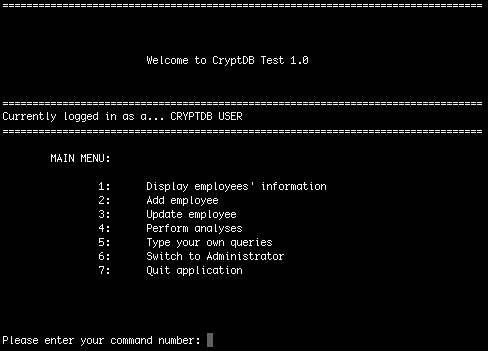
\includegraphics[scale=0.65]{terminal/app_user_mainmenu.png}
	\caption{Main menu for users logged in as CryptDB users, i.e. connecting through the proxy server.}
	\label{fig:app_mm_user}
\end{figure}

When the user selects option 1 in order to show information regarding the employees of the firm, the application sends a \verb!SELECT * FROM employees;! query to the proxy server. As previously explained, the proxy server intercepts the query and anonymizes it. This can be seen in Figure \ref{fig:proxy_enc_res}, which also shows the encrypted result that is returned from the database server. The result is then decrypted and sent to the application, where it is displayed to the user as seen in Figure \ref{fig:app_user_emp}.

\begin{figure}
	\centering
	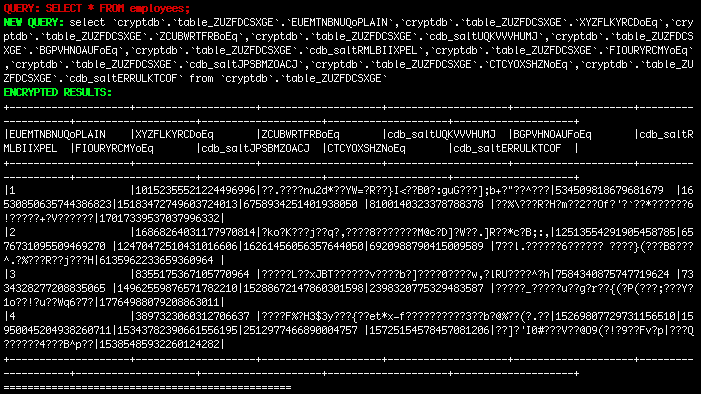
\includegraphics[scale=0.55]{terminal/proxy_enc_res.png}
	\caption{The observed processing at the proxy server when querying information about all employees.}
	\label{fig:proxy_enc_res}
\end{figure}


\begin{figure}
	\centering
	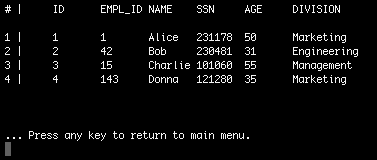
\includegraphics[scale=0.68]{terminal/app_user_emp.png}
	\caption{The result displayed at the CryptDB user when querying for information regarding all employees.}
	\label{fig:app_user_emp}
\end{figure}

%\newpage

\subsection{Confirming the Encrypted Administrator View}

To illustrate the case of the curious database administrator, which is the most easy-to-demonstrate threat, the application has two views. These are the CryptDB user view, and the database administrator view, which can easily be switched between in the application. Depending on whether the application is connected through the proxy or not, the menu items also changes as shown in Figure \ref{fig:app_mm_user} and Figure \ref{fig:app_mm_admin}. Such a switch is performed by simply disconnecting from the application and perform a new log-in on either port 3306 or 3307 based on the previous view. The available menu items depends on the current user's role.


\begin{figure}
	\centering
	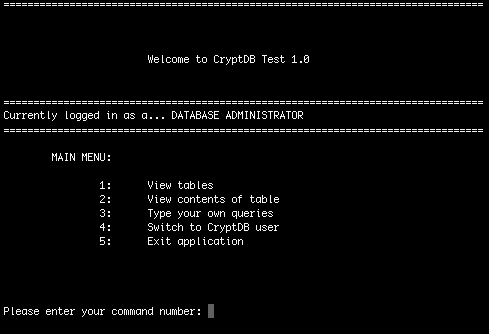
\includegraphics[scale=0.62]{terminal/app_admin_mainmenu.png}
	\caption{Main menu for administrators, i.e. connecting directly to the database server.}
	\label{fig:app_mm_admin}
\end{figure}


\newpage

\begin{wrapfigure}[13]{r}{8cm}
	\centering
    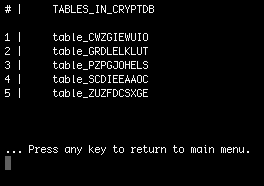
\includegraphics[scale = 0.75]{terminal/app_admin_enc_res1.png}
    \caption{Encrypted tables in CryptDB from a database administrator's perspective.}
    \label{fig:app_admin_enc_res1}
\end{wrapfigure}

For curious database administrators, in addition to performing "free queries", they are also able to view the tables stored in the database, as well as displaying the contents of a table. Remember that one of the key features of CryptDB is that it protects against such curious administrators by encrypting all data inserted in the database.

Figure \ref{fig:app_admin_enc_res1} displays the result when querying the database with the \verb!SHOW TABLES;! statement. All table names are encrypted making it difficult for the administrator to achieve any knowledge about the database. One of the features in the administrator's view is to view the contents of a table, which is done by specifying the name of the table. While the data is encrypted, this does not prevent a curious to perform queries on the encrypted data. For example, there is no obstacles for him to perform a query such as

\begin{verbatim}
SELECT *
FROM table_ZUZFDCSXGE;
\end{verbatim}

But, the resulting data is of course encrypted, and nothing more than obscure symbols are returned. Figure \ref{fig:admin_enc_res2} shows the resulting data to the query above. Note that the only property not to be encrypted is the row id, hence the database administrator is able to find out the number of rows in a table.

\begin{figure}[h]
	\centering
	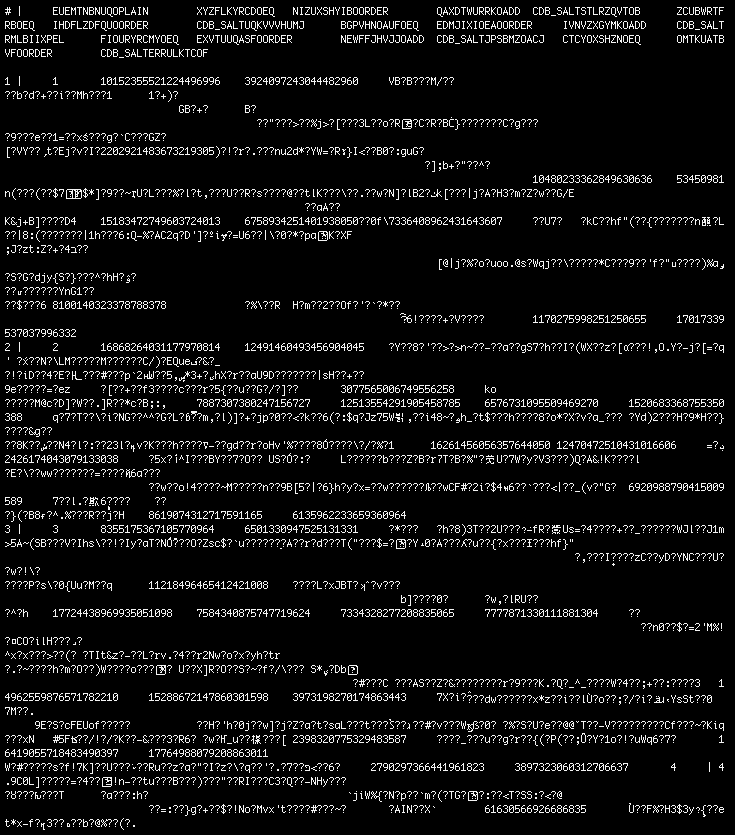
\includegraphics[scale=0.50]{terminal/app_admin_enc_res2.png}
	\caption{Encrypted data observed by the database administrator.}
	\label{fig:admin_enc_res2}
\end{figure}



\newpage
\subsection{Inspecting CryptDB Using DBMS Tools}

Python and MySQLdb does not provide any graphical way to investigate the database server. However, by installing a \gls{dbms} environment such as MySQL Workbench \cite{mysql_workbench}, inspecting the database suddenly becomes possible. MySQL Workbench provides many different features when inspecting databases, all from performing queries on the tables and describing tables and fields, to 
monitoring the database. By simply logging in, the administrator is able to view all tables in the database and inspect them by issuing the \verb!SELECT! query mentioned in the previous section.

\begin{figure}[h]
	\centering
	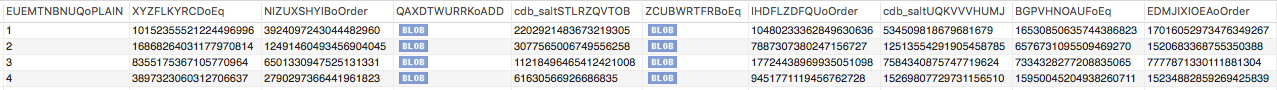
\includegraphics[scale=0.57]{terminal/admin_query_result.png}
	\caption{The resulting rows from performing a SELECT query on the encrypted table. Only the encrypted values of the employee number is shown. Observe that the values are encrypted three times under the different onions Eq, Ord and ADD.}
	\label{fig:admin_query_result}
\end{figure}

As observed, the data is not displayed as random symbols as from the demo application, but rather represented as large integers. It also possible to observe the different onion encryptions of each attribute as they are encrypted as separate columns. By looking very closely at the figure above, it is possible to spot the name of the columns, where the EQ-onion ends with \emph{Eq}, the ORD-onion with \emph{Order} and the ADD-onion with \emph{ADD}. Figure \ref{fig:admin_fields_view} shows a clearer picture of the available information when inspecting tables. The database administrator is able to see the number of columns, and what type of onions the column is encrypted under, as well as their raw types.

\begin{figure}[h]
	\centering
	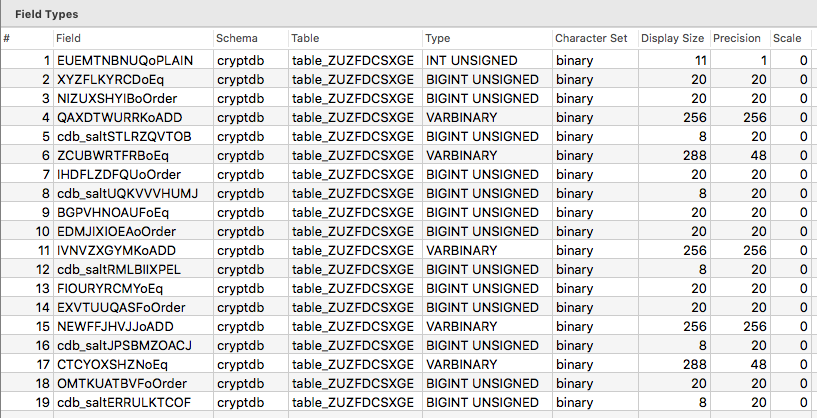
\includegraphics[scale=0.45]{terminal/admin_fields_view.png}
	\caption{Overview of the fields in the encrypted table table\_ZUZFDCSXGE when inspecting the database using MySQL Workbench.}
	\label{fig:admin_fields_view}
\end{figure}

\section{Discussion on CryptDB as a Software}

While being a bit challenging to install and successfully connect to a database system, CryptDB seems to work as intended when operating on encrypted data. What makes CryptDB especially easy to work with is that it is compatible with MySQL, which is a very established and heavily documented \gls{dbms}. This makes it easy and fast to connect CryptDB to existing applications or creating new applications without much knowledge about it. However, the developer should have some insight in what types of operations that are feasible, and how to securely integrate CryptDB without breaking the assumptions and restrictions presented in the recently proposed guidelines \cite{cryptdb_guidelines}. It is clear that CryptDB is not meant for commercial use, both indicated by the lack of documentation and clear guides on implementing applications.

This project has not investigated the overhead when using CryptDB compared to a regular \gls{dbms}, but the developers states that the throughput of CryptDB is 21-26 \% lower than running on a regular MySQL server \citep{CryptDB_Main_Paper}, which seems modest. However, because of lack of time and access to a suitable dataset, this project has not assessed the benchmarks of CryptDB.

The developers have taken the idea further with Mylar \cite{mylar_homepage}, which addresses the threats of attacks on multi-user mode. It is created with the experience from CryptDB in mind, but with focus on running multi-user web applications using the building blocks suggested in CryptDB.

\chapter{Comparison and Conclusion}
\label{chp:conclusion}

This chapter will cover a comparison of CryptDB with a general \gls{fhe} scheme, as well as the conclusion of this project. Finally, the impact and future use cases of CryptDB will be pointed out, along with the possibly future work of this project.

\section{Comparing CryptDB to a Fully Homomorphic Encryption Scheme}

\subsection{Functionality}
As discussed in Section \ref{sec:limits}, CryptDB is subject to some limitations when it comes to functionality. While most of these limitations are possible to avoid by using non-standard approaches or "tweaking" standard queries, it is not true that CryptDB supports all types of operations. Because of these limitations, we can state that CryptDB does not provide functionality of a \gls{fhe} scheme, where we recall that all possible operations on the encrypted data are supported.

\subsection{Security}

CryptDB is based on well-known encryption schemes where the security is tied to well-studied problems being \emph{hard}. \gls{fhe} schemes, however, are based on \emph{newer} hard problems that are not as well-studied as the problems described in Chapter \ref{chp:background}. For example the \gls{lwe} problem (introduced in 2005 \cite{lwe}), which is based on a problem in machine learning, and the Approximate \gls{gcd} problem (introduced in 1985 \cite{app_gcd}) taking advantage of the difficulty of finding the \gls{gcd} of a number given a bunch of near multiples of the number. One can argue if this makes the security of the encryption schemes used in CryptDB stronger than a \gls{fhe} scheme, but the cryptography used in CryptDB is more studied than the cryptography used in today's \gls{fhe} schemes.

\subsection{Performance}

As previously described, one of the biggest weaknesses of \gls{fhe} schemes in today's world, is their impracticality. Especially performance-wise, a \gls{fhe} system spends a tremendous amount of time when processing data in a secure manner. In this category, CryptDB is naturally way ahead of a \gls{fhe} system, as it costs only a reasonable 21-26\% decrease in throughput compared to regular servers running MySQL \cite{CryptDB_Main_Paper}. As the demo application presented has not been exposed to large dataset, it has not been possible to verify the claims presented in the original paper on CryptDB \citep{CryptDB_Main_Paper}.

\section{Conclusion}

This project has been about assessing CryptDB, its main features, and how it works. The results have been an overview of the system and its way of utilizing different types of encryption in order to create a somewhat homomorphic encryption scheme. CryptDB provides a neat software, which is easy to interact with after the installation and set-up has been successful. It comes with a brief "how to install and run" guide available in their GitHub repository. However, this guide may to some seem as a bit vague. Therefore, some of the attention of this project has been given to create a small and easy guide for future projects wishing to explore CryptDB to follow. Along with the assessment, a small demonstration application has been created for testing the various queries that CryptDB allows and to observe the behaviour of the proxy server.


CryptDB certainly provides an interesting approach for practical homomorphic encryption schemes utilizing \gls{sql}. It supports a large set of possible \gls{sql} operations to be performed while both providing confidentiality of the data and being efficient at the same time. However, when seen in connection with the attacks presented in Chapter \ref{chp:attacks}, using CryptDB's approaches may not be the best direction for future implementations of \gls{he} schemes. Especially applications intended for multiple users have been proven to either leak information about data encrypted with weaker encryption scheme, or put possibly destructive restrictions on the developer with respect to usefulness. 

\section{Impact and Future Use of CryptDB}

CryptDB is the first practical implementation of a somewhat homomorphic encryption scheme using \gls{sql}, and has shown a possible approach for creating encrypted databases. A lot of well-known companies such as Google, Microsoft and SAP, as well as a lot of start-ups, are using CrytpDB's building blocks and putting its ideas into their commercial software \cite{cryptdb_homepage}. As CryptDB is enabled exclusively for single-user applications in the nearest future, it is difficult to point out useful applications involving highly sensitive data. The possible weaknesses of CryptDB presented in Chapter \ref{chp:attacks} may indicate that the authors have made the right call when removing the multi-user possibility from CryptDB and recreated its ideas under the new project Mylar \cite{mylar_homepage}.  

However, CryptDB seems to be a well-suited approach for creating diaries, contact lists, and other applications targeted for a single user. One might argue that it may be more convenient for the developer of such applications to use strong encryption, decrypt the queried data at the client side and perform operations on the plaintext. However, leaving sensitive information in plaintext for just a second, gives an attacker a possible window for stealing it. The single-user mode may also be a solution for developers not being able to provide their own servers. By outsourcing the hosting of the application to a cloud service, the developer is able to easily communicate with his application in a confidential and secure manner.

It would have been interesting to create a more comprehensive system and run tests with a large dataset to verify exactly how efficient CryptDB is. Unfortunately, because of the limited amount of time, this is yet to be done. It would also have been interesting to try to recreate the attack proposed by Microsoft Research, if not on a multi-user mode application, then perhaps on a single-user application.




\renewcommand*{\bibname}{References}
\bibliographystyle{acm}
\bibliography{main.bib}

%% Uncomment the following if you have any appendix
% \appendix
% \addtocontents{toc}{%
%  \protect\vspace{1em}% 
%  \protect\noindent \bfseries \appendixtocname\protect\par
%  \protect\vspace{-.5em}%
% }
% \renewcommand{\chaptername}{\appendixname}
%% include below possible appendices (chapters)


\end{document} 
